\documentclass[twoside]{book}

% Packages required by doxygen
\usepackage{fixltx2e}
\usepackage{calc}
\usepackage{doxygen}
\usepackage[export]{adjustbox} % also loads graphicx
\usepackage{graphicx}
\usepackage[utf8]{inputenc}
\usepackage{makeidx}
\usepackage{multicol}
\usepackage{multirow}
\PassOptionsToPackage{warn}{textcomp}
\usepackage{textcomp}
\usepackage[nointegrals]{wasysym}
\usepackage[table]{xcolor}

% Font selection
\usepackage[T1]{fontenc}
\usepackage[scaled=.90]{helvet}
\usepackage{courier}
\usepackage{amssymb}
\usepackage{sectsty}
\renewcommand{\familydefault}{\sfdefault}
\allsectionsfont{%
  \fontseries{bc}\selectfont%
  \color{darkgray}%
}
\renewcommand{\DoxyLabelFont}{%
  \fontseries{bc}\selectfont%
  \color{darkgray}%
}
\newcommand{\+}{\discretionary{\mbox{\scriptsize$\hookleftarrow$}}{}{}}

% Page & text layout
\usepackage{geometry}
\geometry{%
  a4paper,%
  top=2.5cm,%
  bottom=2.5cm,%
  left=2.5cm,%
  right=2.5cm%
}
\tolerance=750
\hfuzz=15pt
\hbadness=750
\setlength{\emergencystretch}{15pt}
\setlength{\parindent}{0cm}
\setlength{\parskip}{3ex plus 2ex minus 2ex}
\makeatletter
\renewcommand{\paragraph}{%
  \@startsection{paragraph}{4}{0ex}{-1.0ex}{1.0ex}{%
    \normalfont\normalsize\bfseries\SS@parafont%
  }%
}
\renewcommand{\subparagraph}{%
  \@startsection{subparagraph}{5}{0ex}{-1.0ex}{1.0ex}{%
    \normalfont\normalsize\bfseries\SS@subparafont%
  }%
}
\makeatother

% Headers & footers
\usepackage{fancyhdr}
\pagestyle{fancyplain}
\fancyhead[LE]{\fancyplain{}{\bfseries\thepage}}
\fancyhead[CE]{\fancyplain{}{}}
\fancyhead[RE]{\fancyplain{}{\bfseries\leftmark}}
\fancyhead[LO]{\fancyplain{}{\bfseries\rightmark}}
\fancyhead[CO]{\fancyplain{}{}}
\fancyhead[RO]{\fancyplain{}{\bfseries\thepage}}
\fancyfoot[LE]{\fancyplain{}{}}
\fancyfoot[CE]{\fancyplain{}{}}
\fancyfoot[RE]{\fancyplain{}{\bfseries\scriptsize Generated by Doxygen }}
\fancyfoot[LO]{\fancyplain{}{\bfseries\scriptsize Generated by Doxygen }}
\fancyfoot[CO]{\fancyplain{}{}}
\fancyfoot[RO]{\fancyplain{}{}}
\renewcommand{\footrulewidth}{0.4pt}
\renewcommand{\chaptermark}[1]{%
  \markboth{#1}{}%
}
\renewcommand{\sectionmark}[1]{%
  \markright{\thesection\ #1}%
}

% Indices & bibliography
\usepackage{natbib}
\usepackage[titles]{tocloft}
\setcounter{tocdepth}{3}
\setcounter{secnumdepth}{5}
\makeindex

% Hyperlinks (required, but should be loaded last)
\usepackage{ifpdf}
\ifpdf
  \usepackage[pdftex,pagebackref=true]{hyperref}
\else
  \usepackage[ps2pdf,pagebackref=true]{hyperref}
\fi
\hypersetup{%
  colorlinks=true,%
  linkcolor=blue,%
  citecolor=blue,%
  unicode%
}

% Custom commands
\newcommand{\clearemptydoublepage}{%
  \newpage{\pagestyle{empty}\cleardoublepage}%
}

\usepackage{caption}
\captionsetup{labelsep=space,justification=centering,font={bf},singlelinecheck=off,skip=4pt,position=top}

%===== C O N T E N T S =====

\begin{document}

% Titlepage & ToC
\hypersetup{pageanchor=false,
             bookmarksnumbered=true,
             pdfencoding=unicode
            }
\pagenumbering{alph}
\begin{titlepage}
\vspace*{7cm}
\begin{center}%
{\Large My Project }\\
\vspace*{1cm}
{\large Generated by Doxygen 1.8.14}\\
\end{center}
\end{titlepage}
\clearemptydoublepage
\pagenumbering{roman}
\tableofcontents
\clearemptydoublepage
\pagenumbering{arabic}
\hypersetup{pageanchor=true}

%--- Begin generated contents ---
\chapter{Class Index}
\section{Class List}
Here are the classes, structs, unions and interfaces with brief descriptions\+:\begin{DoxyCompactList}
\item\contentsline{section}{\mbox{\hyperlink{classaxis}{axis}} }{\pageref{classaxis}}{}
\item\contentsline{section}{\mbox{\hyperlink{classedge2_d}{edge2D}} }{\pageref{classedge2_d}}{}
\item\contentsline{section}{\mbox{\hyperlink{classedge3_d}{edge3D}} }{\pageref{classedge3_d}}{}
\item\contentsline{section}{\mbox{\hyperlink{class_face}{Face}} }{\pageref{class_face}}{}
\item\contentsline{section}{\mbox{\hyperlink{classobject}{object}} }{\pageref{classobject}}{}
\item\contentsline{section}{\mbox{\hyperlink{classvertex2_d}{vertex2D}} }{\pageref{classvertex2_d}}{}
\item\contentsline{section}{\mbox{\hyperlink{classview2_d}{view2D}} }{\pageref{classview2_d}}{}
\item\contentsline{section}{\mbox{\hyperlink{classview3_d}{view3D}} }{\pageref{classview3_d}}{}
\end{DoxyCompactList}

\chapter{File Index}
\section{File List}
Here is a list of all files with brief descriptions\+:\begin{DoxyCompactList}
\item\contentsline{section}{\mbox{\hyperlink{classes_8h}{classes.\+h}} }{\pageref{classes_8h}}{}
\item\contentsline{section}{\mbox{\hyperlink{conversion_8cpp}{conversion.\+cpp}} }{\pageref{conversion_8cpp}}{}
\item\contentsline{section}{\mbox{\hyperlink{main_8cpp}{main.\+cpp}} }{\pageref{main_8cpp}}{}
\item\contentsline{section}{\mbox{\hyperlink{primitive_8h}{primitive.\+h}} }{\pageref{primitive_8h}}{}
\item\contentsline{section}{\mbox{\hyperlink{transformations2_d_8cpp}{transformations2\+D.\+cpp}} }{\pageref{transformations2_d_8cpp}}{}
\item\contentsline{section}{\mbox{\hyperlink{transformations3_d_8cpp}{transformations3\+D.\+cpp}} }{\pageref{transformations3_d_8cpp}}{}
\end{DoxyCompactList}

\chapter{Class Documentation}
\hypertarget{classaxis}{}\section{axis Class Reference}
\label{classaxis}\index{axis@{axis}}


{\ttfamily \#include $<$primitive.\+h$>$}



Collaboration diagram for axis\+:
\nopagebreak
\begin{figure}[H]
\begin{center}
\leavevmode
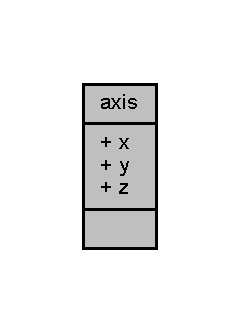
\includegraphics[width=115pt]{classaxis__coll__graph}
\end{center}
\end{figure}
\subsection*{Public Attributes}
\begin{DoxyCompactItemize}
\item 
double \mbox{\hyperlink{classaxis_a3dbf8b803298595013fd5d6d639a930f}{x}}
\item 
double \mbox{\hyperlink{classaxis_ad2d7e25ee425fee3ee7e818839897ab9}{y}}
\item 
double \mbox{\hyperlink{classaxis_aacda2920117dea5bca43044c368805d6}{z}}
\end{DoxyCompactItemize}


\subsection{Member Data Documentation}
\mbox{\Hypertarget{classaxis_a3dbf8b803298595013fd5d6d639a930f}\label{classaxis_a3dbf8b803298595013fd5d6d639a930f}} 
\index{axis@{axis}!x@{x}}
\index{x@{x}!axis@{axis}}
\subsubsection{\texorpdfstring{x}{x}}
{\footnotesize\ttfamily double axis\+::x}

\mbox{\Hypertarget{classaxis_ad2d7e25ee425fee3ee7e818839897ab9}\label{classaxis_ad2d7e25ee425fee3ee7e818839897ab9}} 
\index{axis@{axis}!y@{y}}
\index{y@{y}!axis@{axis}}
\subsubsection{\texorpdfstring{y}{y}}
{\footnotesize\ttfamily double axis\+::y}

\mbox{\Hypertarget{classaxis_aacda2920117dea5bca43044c368805d6}\label{classaxis_aacda2920117dea5bca43044c368805d6}} 
\index{axis@{axis}!z@{z}}
\index{z@{z}!axis@{axis}}
\subsubsection{\texorpdfstring{z}{z}}
{\footnotesize\ttfamily double axis\+::z}



The documentation for this class was generated from the following file\+:\begin{DoxyCompactItemize}
\item 
\mbox{\hyperlink{primitive_8h}{primitive.\+h}}\end{DoxyCompactItemize}

\hypertarget{classedge2_d}{}\section{edge2D Class Reference}
\label{classedge2_d}\index{edge2D@{edge2D}}


{\ttfamily \#include $<$primitive.\+h$>$}



Collaboration diagram for edge2D\+:
\nopagebreak
\begin{figure}[H]
\begin{center}
\leavevmode
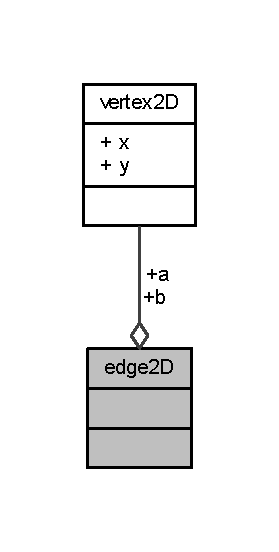
\includegraphics[width=134pt]{classedge2_d__coll__graph}
\end{center}
\end{figure}
\subsection*{Public Attributes}
\begin{DoxyCompactItemize}
\item 
\mbox{\hyperlink{classvertex2_d}{vertex2D}} \mbox{\hyperlink{classedge2_d_a2f62b09a7626de5187523ecc359487fd}{a}}
\item 
\mbox{\hyperlink{classvertex2_d}{vertex2D}} \mbox{\hyperlink{classedge2_d_a34a5d6f487b0935992736b14ef7abe21}{b}}
\end{DoxyCompactItemize}


\subsection{Member Data Documentation}
\mbox{\Hypertarget{classedge2_d_a2f62b09a7626de5187523ecc359487fd}\label{classedge2_d_a2f62b09a7626de5187523ecc359487fd}} 
\index{edge2D@{edge2D}!a@{a}}
\index{a@{a}!edge2D@{edge2D}}
\subsubsection{\texorpdfstring{a}{a}}
{\footnotesize\ttfamily \mbox{\hyperlink{classvertex2_d}{vertex2D}} edge2\+D\+::a}

\mbox{\Hypertarget{classedge2_d_a34a5d6f487b0935992736b14ef7abe21}\label{classedge2_d_a34a5d6f487b0935992736b14ef7abe21}} 
\index{edge2D@{edge2D}!b@{b}}
\index{b@{b}!edge2D@{edge2D}}
\subsubsection{\texorpdfstring{b}{b}}
{\footnotesize\ttfamily \mbox{\hyperlink{classvertex2_d}{vertex2D}} edge2\+D\+::b}



The documentation for this class was generated from the following file\+:\begin{DoxyCompactItemize}
\item 
\mbox{\hyperlink{primitive_8h}{primitive.\+h}}\end{DoxyCompactItemize}

\hypertarget{classedge3_d}{}\section{edge3D Class Reference}
\label{classedge3_d}\index{edge3D@{edge3D}}


{\ttfamily \#include $<$primitive.\+h$>$}



Collaboration diagram for edge3D\+:
\nopagebreak
\begin{figure}[H]
\begin{center}
\leavevmode
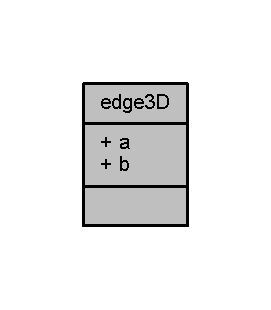
\includegraphics[width=130pt]{classedge3_d__coll__graph}
\end{center}
\end{figure}
\subsection*{Public Attributes}
\begin{DoxyCompactItemize}
\item 
vertex3D \mbox{\hyperlink{classedge3_d_ac6e93edf5cf00d4f5384c747aa0e881f}{a}}
\item 
vertex3D \mbox{\hyperlink{classedge3_d_a2b8676adbcd52863011450e35c16f79b}{b}}
\end{DoxyCompactItemize}


\subsection{Member Data Documentation}
\mbox{\Hypertarget{classedge3_d_ac6e93edf5cf00d4f5384c747aa0e881f}\label{classedge3_d_ac6e93edf5cf00d4f5384c747aa0e881f}} 
\index{edge3D@{edge3D}!a@{a}}
\index{a@{a}!edge3D@{edge3D}}
\subsubsection{\texorpdfstring{a}{a}}
{\footnotesize\ttfamily vertex3D edge3\+D\+::a}

\mbox{\Hypertarget{classedge3_d_a2b8676adbcd52863011450e35c16f79b}\label{classedge3_d_a2b8676adbcd52863011450e35c16f79b}} 
\index{edge3D@{edge3D}!b@{b}}
\index{b@{b}!edge3D@{edge3D}}
\subsubsection{\texorpdfstring{b}{b}}
{\footnotesize\ttfamily vertex3D edge3\+D\+::b}



The documentation for this class was generated from the following file\+:\begin{DoxyCompactItemize}
\item 
\mbox{\hyperlink{primitive_8h}{primitive.\+h}}\end{DoxyCompactItemize}

\hypertarget{class_face}{}\section{Face Class Reference}
\label{class_face}\index{Face@{Face}}


{\ttfamily \#include $<$primitive.\+h$>$}



Collaboration diagram for Face\+:
\nopagebreak
\begin{figure}[H]
\begin{center}
\leavevmode
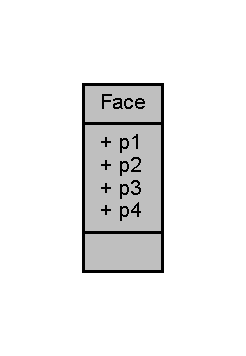
\includegraphics[width=118pt]{class_face__coll__graph}
\end{center}
\end{figure}
\subsection*{Public Attributes}
\begin{DoxyCompactItemize}
\item 
vertex3D \mbox{\hyperlink{class_face_ad0c1698c5f8281fc3f3d3e5d12ff6ac4}{p1}}
\item 
vertex3D \mbox{\hyperlink{class_face_aa7c7c6a437774d7ff2c95fdc96ad7840}{p2}}
\item 
vertex3D \mbox{\hyperlink{class_face_a83603534660d5aea15b287d83b0aa2d8}{p3}}
\item 
vertex3D \mbox{\hyperlink{class_face_a0691e5c72ca6be50acb683e12ce1482f}{p4}}
\end{DoxyCompactItemize}


\subsection{Member Data Documentation}
\mbox{\Hypertarget{class_face_ad0c1698c5f8281fc3f3d3e5d12ff6ac4}\label{class_face_ad0c1698c5f8281fc3f3d3e5d12ff6ac4}} 
\index{Face@{Face}!p1@{p1}}
\index{p1@{p1}!Face@{Face}}
\subsubsection{\texorpdfstring{p1}{p1}}
{\footnotesize\ttfamily vertex3D Face\+::p1}

\mbox{\Hypertarget{class_face_aa7c7c6a437774d7ff2c95fdc96ad7840}\label{class_face_aa7c7c6a437774d7ff2c95fdc96ad7840}} 
\index{Face@{Face}!p2@{p2}}
\index{p2@{p2}!Face@{Face}}
\subsubsection{\texorpdfstring{p2}{p2}}
{\footnotesize\ttfamily vertex3D Face\+::p2}

\mbox{\Hypertarget{class_face_a83603534660d5aea15b287d83b0aa2d8}\label{class_face_a83603534660d5aea15b287d83b0aa2d8}} 
\index{Face@{Face}!p3@{p3}}
\index{p3@{p3}!Face@{Face}}
\subsubsection{\texorpdfstring{p3}{p3}}
{\footnotesize\ttfamily vertex3D Face\+::p3}

\mbox{\Hypertarget{class_face_a0691e5c72ca6be50acb683e12ce1482f}\label{class_face_a0691e5c72ca6be50acb683e12ce1482f}} 
\index{Face@{Face}!p4@{p4}}
\index{p4@{p4}!Face@{Face}}
\subsubsection{\texorpdfstring{p4}{p4}}
{\footnotesize\ttfamily vertex3D Face\+::p4}



The documentation for this class was generated from the following file\+:\begin{DoxyCompactItemize}
\item 
\mbox{\hyperlink{primitive_8h}{primitive.\+h}}\end{DoxyCompactItemize}

\hypertarget{classobject}{}\section{object Class Reference}
\label{classobject}\index{object@{object}}


{\ttfamily \#include $<$classes.\+h$>$}



Collaboration diagram for object\+:
\nopagebreak
\begin{figure}[H]
\begin{center}
\leavevmode
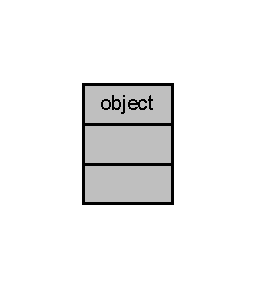
\includegraphics[width=123pt]{classobject__coll__graph}
\end{center}
\end{figure}


The documentation for this class was generated from the following file\+:\begin{DoxyCompactItemize}
\item 
\mbox{\hyperlink{classes_8h}{classes.\+h}}\end{DoxyCompactItemize}

\hypertarget{classvertex2_d}{}\section{vertex2D Class Reference}
\label{classvertex2_d}\index{vertex2D@{vertex2D}}


{\ttfamily \#include $<$primitive.\+h$>$}



Collaboration diagram for vertex2D\+:
\nopagebreak
\begin{figure}[H]
\begin{center}
\leavevmode
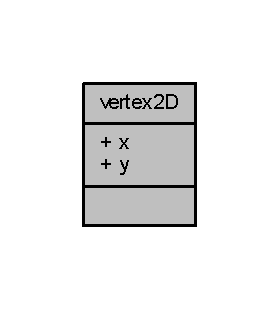
\includegraphics[width=134pt]{classvertex2_d__coll__graph}
\end{center}
\end{figure}
\subsection*{Public Attributes}
\begin{DoxyCompactItemize}
\item 
double \mbox{\hyperlink{classvertex2_d_a0022f681a4ded8ba4c741b461a6944eb}{x}}
\item 
double \mbox{\hyperlink{classvertex2_d_aaa0010f8b85b5837db64ef78f8151afe}{y}}
\end{DoxyCompactItemize}


\subsection{Member Data Documentation}
\mbox{\Hypertarget{classvertex2_d_a0022f681a4ded8ba4c741b461a6944eb}\label{classvertex2_d_a0022f681a4ded8ba4c741b461a6944eb}} 
\index{vertex2D@{vertex2D}!x@{x}}
\index{x@{x}!vertex2D@{vertex2D}}
\subsubsection{\texorpdfstring{x}{x}}
{\footnotesize\ttfamily double vertex2\+D\+::x}

\mbox{\Hypertarget{classvertex2_d_aaa0010f8b85b5837db64ef78f8151afe}\label{classvertex2_d_aaa0010f8b85b5837db64ef78f8151afe}} 
\index{vertex2D@{vertex2D}!y@{y}}
\index{y@{y}!vertex2D@{vertex2D}}
\subsubsection{\texorpdfstring{y}{y}}
{\footnotesize\ttfamily double vertex2\+D\+::y}



The documentation for this class was generated from the following file\+:\begin{DoxyCompactItemize}
\item 
\mbox{\hyperlink{primitive_8h}{primitive.\+h}}\end{DoxyCompactItemize}

\hypertarget{classview2_d}{}\section{view2D Class Reference}
\label{classview2_d}\index{view2D@{view2D}}


{\ttfamily \#include $<$primitive.\+h$>$}



Collaboration diagram for view2D\+:
\nopagebreak
\begin{figure}[H]
\begin{center}
\leavevmode
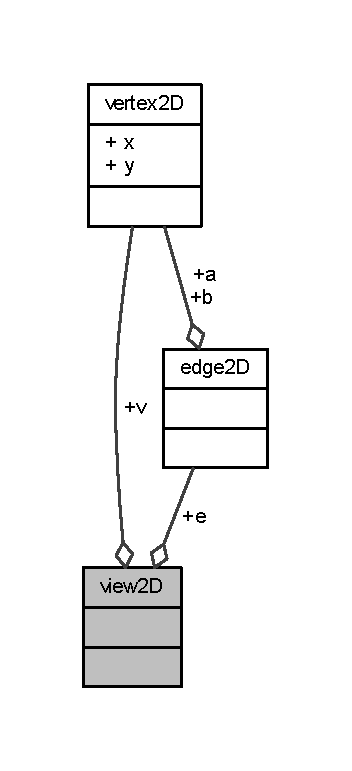
\includegraphics[width=169pt]{classview2_d__coll__graph}
\end{center}
\end{figure}
\subsection*{Public Attributes}
\begin{DoxyCompactItemize}
\item 
\mbox{\hyperlink{classvertex2_d}{vertex2D}} \mbox{[}$\,$\mbox{]} \mbox{\hyperlink{classview2_d_abde5a351bf6796ae8149a3f00a783caa}{v}}
\item 
\mbox{\hyperlink{classedge2_d}{edge2D}} \mbox{[}$\,$\mbox{]} \mbox{\hyperlink{classview2_d_a3a6ad7e000ebbcf7caefe3767dfc036b}{e}}
\end{DoxyCompactItemize}


\subsection{Member Data Documentation}
\mbox{\Hypertarget{classview2_d_a3a6ad7e000ebbcf7caefe3767dfc036b}\label{classview2_d_a3a6ad7e000ebbcf7caefe3767dfc036b}} 
\index{view2D@{view2D}!e@{e}}
\index{e@{e}!view2D@{view2D}}
\subsubsection{\texorpdfstring{e}{e}}
{\footnotesize\ttfamily \mbox{\hyperlink{classedge2_d}{edge2D}} \mbox{[}$\,$\mbox{]} view2\+D\+::e}

\mbox{\Hypertarget{classview2_d_abde5a351bf6796ae8149a3f00a783caa}\label{classview2_d_abde5a351bf6796ae8149a3f00a783caa}} 
\index{view2D@{view2D}!v@{v}}
\index{v@{v}!view2D@{view2D}}
\subsubsection{\texorpdfstring{v}{v}}
{\footnotesize\ttfamily \mbox{\hyperlink{classvertex2_d}{vertex2D}} \mbox{[}$\,$\mbox{]} view2\+D\+::v}



The documentation for this class was generated from the following file\+:\begin{DoxyCompactItemize}
\item 
\mbox{\hyperlink{primitive_8h}{primitive.\+h}}\end{DoxyCompactItemize}

\hypertarget{classview3_d}{}\section{view3D Class Reference}
\label{classview3_d}\index{view3D@{view3D}}


{\ttfamily \#include $<$primitive.\+h$>$}



Collaboration diagram for view3D\+:
\nopagebreak
\begin{figure}[H]
\begin{center}
\leavevmode
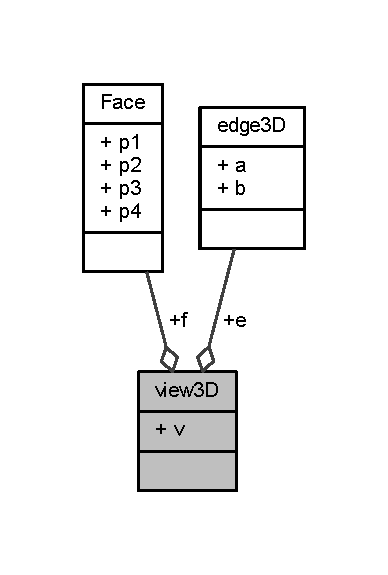
\includegraphics[width=186pt]{classview3_d__coll__graph}
\end{center}
\end{figure}
\subsection*{Public Attributes}
\begin{DoxyCompactItemize}
\item 
vertex3D \mbox{[}$\,$\mbox{]} \mbox{\hyperlink{classview3_d_a6a7f3e82c10b2c7476ffd8be0d3ecee2}{v}}
\item 
\mbox{\hyperlink{classedge3_d}{edge3D}} \mbox{[}$\,$\mbox{]} \mbox{\hyperlink{classview3_d_a1aa4051bc2abc3748148b2f1dfd036db}{e}}
\item 
\mbox{\hyperlink{class_face}{Face}} \mbox{[}$\,$\mbox{]} \mbox{\hyperlink{classview3_d_af8d43cfca632dd12bdb5eb8558b8ae62}{f}}
\end{DoxyCompactItemize}


\subsection{Member Data Documentation}
\mbox{\Hypertarget{classview3_d_a1aa4051bc2abc3748148b2f1dfd036db}\label{classview3_d_a1aa4051bc2abc3748148b2f1dfd036db}} 
\index{view3D@{view3D}!e@{e}}
\index{e@{e}!view3D@{view3D}}
\subsubsection{\texorpdfstring{e}{e}}
{\footnotesize\ttfamily \mbox{\hyperlink{classedge3_d}{edge3D}} \mbox{[}$\,$\mbox{]} view3\+D\+::e}

\mbox{\Hypertarget{classview3_d_af8d43cfca632dd12bdb5eb8558b8ae62}\label{classview3_d_af8d43cfca632dd12bdb5eb8558b8ae62}} 
\index{view3D@{view3D}!f@{f}}
\index{f@{f}!view3D@{view3D}}
\subsubsection{\texorpdfstring{f}{f}}
{\footnotesize\ttfamily \mbox{\hyperlink{class_face}{Face}} \mbox{[}$\,$\mbox{]} view3\+D\+::f}

\mbox{\Hypertarget{classview3_d_a6a7f3e82c10b2c7476ffd8be0d3ecee2}\label{classview3_d_a6a7f3e82c10b2c7476ffd8be0d3ecee2}} 
\index{view3D@{view3D}!v@{v}}
\index{v@{v}!view3D@{view3D}}
\subsubsection{\texorpdfstring{v}{v}}
{\footnotesize\ttfamily vertex3D \mbox{[}$\,$\mbox{]} view3\+D\+::v}



The documentation for this class was generated from the following file\+:\begin{DoxyCompactItemize}
\item 
\mbox{\hyperlink{primitive_8h}{primitive.\+h}}\end{DoxyCompactItemize}

\chapter{File Documentation}
\hypertarget{classes_8h}{}\section{classes.\+h File Reference}
\label{classes_8h}\index{classes.\+h@{classes.\+h}}
{\ttfamily \#include \char`\"{}primitive.\+h\char`\"{}}\newline
Include dependency graph for classes.\+h\+:
\nopagebreak
\begin{figure}[H]
\begin{center}
\leavevmode
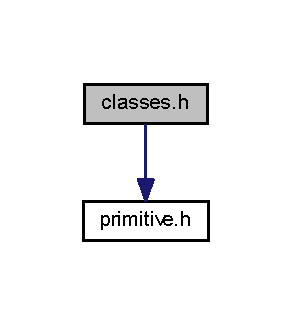
\includegraphics[width=140pt]{classes_8h__incl}
\end{center}
\end{figure}
This graph shows which files directly or indirectly include this file\+:
\nopagebreak
\begin{figure}[H]
\begin{center}
\leavevmode
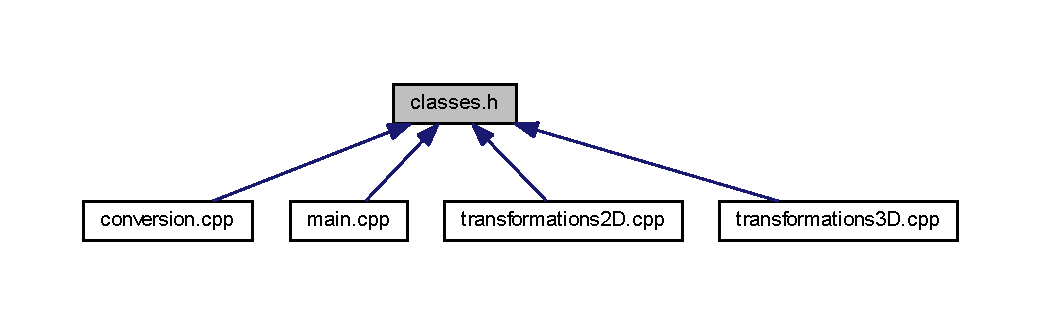
\includegraphics[width=350pt]{classes_8h__dep__incl}
\end{center}
\end{figure}
\subsection*{Classes}
\begin{DoxyCompactItemize}
\item 
class \mbox{\hyperlink{classobject}{object}}
\end{DoxyCompactItemize}
\subsection*{Functions}
\begin{DoxyCompactItemize}
\item 
\mbox{\hyperlink{classobject}{object}} \mbox{\hyperlink{classes_8h_a6d172d5c6754ca0c9a657d3705ff765d}{Generate3D}} (\mbox{\hyperlink{classview2_d}{view2D}} a, \mbox{\hyperlink{classview2_d}{view2D}} b, \mbox{\hyperlink{classview2_d}{view2D}} c)
\item 
\mbox{\hyperlink{classview2_d}{view2D}} \mbox{\hyperlink{classes_8h_a6ca40087d9625015aa7c6ec2ed6af462}{translate2D}} (\mbox{\hyperlink{classview2_d}{view2D}} a, double \mbox{\hyperlink{primitive_8h_a521441fc7ec247d21ca8c376f778ff08}{x}}, double \mbox{\hyperlink{primitive_8h_a5e287957a4fe616e55aa59c129f49a92}{y}})
\item 
\mbox{\hyperlink{classview2_d}{view2D}} \mbox{\hyperlink{classes_8h_a05ac14eedc523383b0f5d4ebba6a5e6d}{scaling2D}} (\mbox{\hyperlink{classview2_d}{view2D}} a, double \mbox{\hyperlink{primitive_8h_a521441fc7ec247d21ca8c376f778ff08}{x}}, double \mbox{\hyperlink{primitive_8h_a5e287957a4fe616e55aa59c129f49a92}{y}})
\item 
\mbox{\hyperlink{classview2_d}{view2D}} \mbox{\hyperlink{classes_8h_ac598e3f9c6a0447bbd970bba10556b07}{rotation2D}} (\mbox{\hyperlink{classview2_d}{view2D}} a, int b, double c)
\end{DoxyCompactItemize}


\subsection{Function Documentation}
\mbox{\Hypertarget{classes_8h_a6d172d5c6754ca0c9a657d3705ff765d}\label{classes_8h_a6d172d5c6754ca0c9a657d3705ff765d}} 
\index{classes.\+h@{classes.\+h}!Generate3D@{Generate3D}}
\index{Generate3D@{Generate3D}!classes.\+h@{classes.\+h}}
\subsubsection{\texorpdfstring{Generate3\+D()}{Generate3D()}}
{\footnotesize\ttfamily \mbox{\hyperlink{classobject}{object}} Generate3D (\begin{DoxyParamCaption}\item[{\mbox{\hyperlink{classview2_d}{view2D}}}]{a,  }\item[{\mbox{\hyperlink{classview2_d}{view2D}}}]{b,  }\item[{\mbox{\hyperlink{classview2_d}{view2D}}}]{c }\end{DoxyParamCaption})}

\mbox{\Hypertarget{classes_8h_ac598e3f9c6a0447bbd970bba10556b07}\label{classes_8h_ac598e3f9c6a0447bbd970bba10556b07}} 
\index{classes.\+h@{classes.\+h}!rotation2D@{rotation2D}}
\index{rotation2D@{rotation2D}!classes.\+h@{classes.\+h}}
\subsubsection{\texorpdfstring{rotation2\+D()}{rotation2D()}}
{\footnotesize\ttfamily \mbox{\hyperlink{classview2_d}{view2D}} rotation2D (\begin{DoxyParamCaption}\item[{\mbox{\hyperlink{classview2_d}{view2D}}}]{a,  }\item[{int}]{b,  }\item[{double}]{c }\end{DoxyParamCaption})}

\mbox{\Hypertarget{classes_8h_a05ac14eedc523383b0f5d4ebba6a5e6d}\label{classes_8h_a05ac14eedc523383b0f5d4ebba6a5e6d}} 
\index{classes.\+h@{classes.\+h}!scaling2D@{scaling2D}}
\index{scaling2D@{scaling2D}!classes.\+h@{classes.\+h}}
\subsubsection{\texorpdfstring{scaling2\+D()}{scaling2D()}}
{\footnotesize\ttfamily \mbox{\hyperlink{classview2_d}{view2D}} scaling2D (\begin{DoxyParamCaption}\item[{\mbox{\hyperlink{classview2_d}{view2D}}}]{a,  }\item[{double}]{x,  }\item[{double}]{y }\end{DoxyParamCaption})}

\mbox{\Hypertarget{classes_8h_a6ca40087d9625015aa7c6ec2ed6af462}\label{classes_8h_a6ca40087d9625015aa7c6ec2ed6af462}} 
\index{classes.\+h@{classes.\+h}!translate2D@{translate2D}}
\index{translate2D@{translate2D}!classes.\+h@{classes.\+h}}
\subsubsection{\texorpdfstring{translate2\+D()}{translate2D()}}
{\footnotesize\ttfamily \mbox{\hyperlink{classview2_d}{view2D}} translate2D (\begin{DoxyParamCaption}\item[{\mbox{\hyperlink{classview2_d}{view2D}}}]{a,  }\item[{double}]{x,  }\item[{double}]{y }\end{DoxyParamCaption})}


\hypertarget{conversion_8cpp}{}\section{conversion.\+cpp File Reference}
\label{conversion_8cpp}\index{conversion.\+cpp@{conversion.\+cpp}}
{\ttfamily \#include \char`\"{}classes.\+h\char`\"{}}\newline
{\ttfamily \#include \char`\"{}primitive.\+h\char`\"{}}\newline
Include dependency graph for conversion.\+cpp\+:
\nopagebreak
\begin{figure}[H]
\begin{center}
\leavevmode
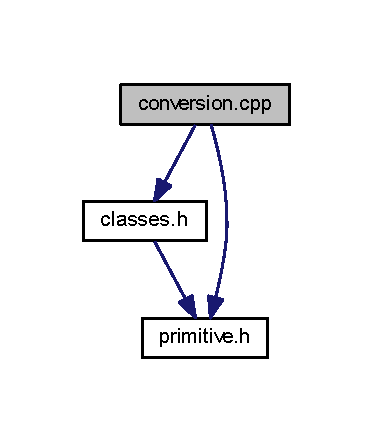
\includegraphics[width=179pt]{conversion_8cpp__incl}
\end{center}
\end{figure}
\subsection*{Functions}
\begin{DoxyCompactItemize}
\item 
\mbox{\hyperlink{classview2_d}{view2D}} \mbox{\hyperlink{conversion_8cpp_af755c3abc8b4cd441746346f4aadc1fc}{Generate2D}} (\mbox{\hyperlink{classobject}{object}} a, double \mbox{\hyperlink{primitive_8h_a521441fc7ec247d21ca8c376f778ff08}{x}}, double \mbox{\hyperlink{primitive_8h_a5e287957a4fe616e55aa59c129f49a92}{y}}, double \mbox{\hyperlink{primitive_8h_aa4b230975c7672e64e45f871e10cddc1}{z}})
\item 
\mbox{\hyperlink{classview2_d}{view2D}} \mbox{[}$\,$\mbox{]} \mbox{\hyperlink{conversion_8cpp_ab732d8648dca292f5c6d03d3c8974783}{orthographic\+Views}} (\mbox{\hyperlink{classobject}{object}} a)
\item 
\mbox{\hyperlink{classobject}{object}} \mbox{\hyperlink{conversion_8cpp_a6d172d5c6754ca0c9a657d3705ff765d}{Generate3D}} (\mbox{\hyperlink{classview2_d}{view2D}} a, \mbox{\hyperlink{classview2_d}{view2D}} b, \mbox{\hyperlink{classview2_d}{view2D}} c)
\end{DoxyCompactItemize}


\subsection{Function Documentation}
\mbox{\Hypertarget{conversion_8cpp_af755c3abc8b4cd441746346f4aadc1fc}\label{conversion_8cpp_af755c3abc8b4cd441746346f4aadc1fc}} 
\index{conversion.\+cpp@{conversion.\+cpp}!Generate2D@{Generate2D}}
\index{Generate2D@{Generate2D}!conversion.\+cpp@{conversion.\+cpp}}
\subsubsection{\texorpdfstring{Generate2\+D()}{Generate2D()}}
{\footnotesize\ttfamily \mbox{\hyperlink{classview2_d}{view2D}} Generate2D (\begin{DoxyParamCaption}\item[{\mbox{\hyperlink{classobject}{object}}}]{a,  }\item[{double}]{x,  }\item[{double}]{y,  }\item[{double}]{z }\end{DoxyParamCaption})}

\mbox{\Hypertarget{conversion_8cpp_a6d172d5c6754ca0c9a657d3705ff765d}\label{conversion_8cpp_a6d172d5c6754ca0c9a657d3705ff765d}} 
\index{conversion.\+cpp@{conversion.\+cpp}!Generate3D@{Generate3D}}
\index{Generate3D@{Generate3D}!conversion.\+cpp@{conversion.\+cpp}}
\subsubsection{\texorpdfstring{Generate3\+D()}{Generate3D()}}
{\footnotesize\ttfamily \mbox{\hyperlink{classobject}{object}} Generate3D (\begin{DoxyParamCaption}\item[{\mbox{\hyperlink{classview2_d}{view2D}}}]{a,  }\item[{\mbox{\hyperlink{classview2_d}{view2D}}}]{b,  }\item[{\mbox{\hyperlink{classview2_d}{view2D}}}]{c }\end{DoxyParamCaption})}

\mbox{\Hypertarget{conversion_8cpp_ab732d8648dca292f5c6d03d3c8974783}\label{conversion_8cpp_ab732d8648dca292f5c6d03d3c8974783}} 
\index{conversion.\+cpp@{conversion.\+cpp}!orthographic\+Views@{orthographic\+Views}}
\index{orthographic\+Views@{orthographic\+Views}!conversion.\+cpp@{conversion.\+cpp}}
\subsubsection{\texorpdfstring{orthographic\+Views()}{orthographicViews()}}
{\footnotesize\ttfamily \mbox{\hyperlink{classview2_d}{view2D}} \mbox{[}$\,$\mbox{]} orthographic\+Views (\begin{DoxyParamCaption}\item[{\mbox{\hyperlink{classobject}{object}}}]{a }\end{DoxyParamCaption})}


\hypertarget{main_8cpp}{}\section{main.\+cpp File Reference}
\label{main_8cpp}\index{main.\+cpp@{main.\+cpp}}
{\ttfamily \#include \char`\"{}primitive.\+h\char`\"{}}\newline
{\ttfamily \#include \char`\"{}classes.\+h\char`\"{}}\newline
Include dependency graph for main.\+cpp\+:
\nopagebreak
\begin{figure}[H]
\begin{center}
\leavevmode
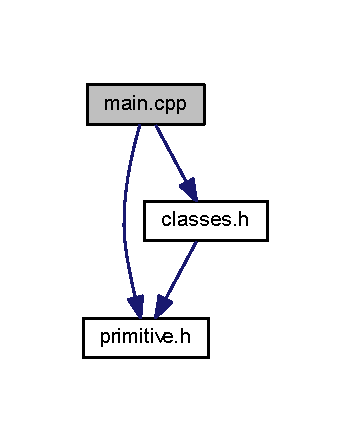
\includegraphics[width=169pt]{main_8cpp__incl}
\end{center}
\end{figure}
\subsection*{Functions}
\begin{DoxyCompactItemize}
\item 
int \mbox{\hyperlink{main_8cpp_ae66f6b31b5ad750f1fe042a706a4e3d4}{main}} ()
\end{DoxyCompactItemize}


\subsection{Function Documentation}
\mbox{\Hypertarget{main_8cpp_ae66f6b31b5ad750f1fe042a706a4e3d4}\label{main_8cpp_ae66f6b31b5ad750f1fe042a706a4e3d4}} 
\index{main.\+cpp@{main.\+cpp}!main@{main}}
\index{main@{main}!main.\+cpp@{main.\+cpp}}
\subsubsection{\texorpdfstring{main()}{main()}}
{\footnotesize\ttfamily int main (\begin{DoxyParamCaption}{ }\end{DoxyParamCaption})}


\hypertarget{primitive_8h}{}\section{primitive.\+h File Reference}
\label{primitive_8h}\index{primitive.\+h@{primitive.\+h}}
This graph shows which files directly or indirectly include this file\+:
\nopagebreak
\begin{figure}[H]
\begin{center}
\leavevmode
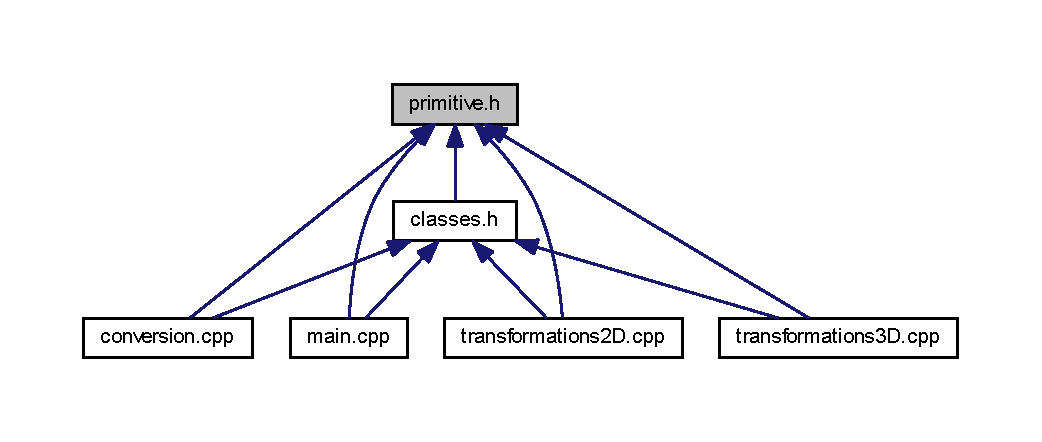
\includegraphics[width=350pt]{primitive_8h__dep__incl}
\end{center}
\end{figure}
\subsection*{Classes}
\begin{DoxyCompactItemize}
\item 
class \mbox{\hyperlink{classvertex2_d}{vertex2D}}
\item 
class \mbox{\hyperlink{classaxis}{axis}}
\item 
class \mbox{\hyperlink{classedge2_d}{edge2D}}
\item 
class \mbox{\hyperlink{classedge3_d}{edge3D}}
\item 
class \mbox{\hyperlink{class_face}{Face}}
\item 
class \mbox{\hyperlink{classview2_d}{view2D}}
\item 
class \mbox{\hyperlink{classview3_d}{view3D}}
\end{DoxyCompactItemize}
\subsection*{Variables}
\begin{DoxyCompactItemize}
\item 
class \mbox{\hyperlink{classaxis}{axis}} \mbox{\hyperlink{primitive_8h_a521441fc7ec247d21ca8c376f778ff08}{x}}
\item 
class \mbox{\hyperlink{classaxis}{axis}} \mbox{\hyperlink{primitive_8h_a5e287957a4fe616e55aa59c129f49a92}{y}}
\item 
class \mbox{\hyperlink{classaxis}{axis}} \mbox{\hyperlink{primitive_8h_aa4b230975c7672e64e45f871e10cddc1}{z}}
\end{DoxyCompactItemize}


\subsection{Variable Documentation}
\mbox{\Hypertarget{primitive_8h_a521441fc7ec247d21ca8c376f778ff08}\label{primitive_8h_a521441fc7ec247d21ca8c376f778ff08}} 
\index{primitive.\+h@{primitive.\+h}!x@{x}}
\index{x@{x}!primitive.\+h@{primitive.\+h}}
\subsubsection{\texorpdfstring{x}{x}}
{\footnotesize\ttfamily class \mbox{\hyperlink{classaxis}{axis}} x}

\mbox{\Hypertarget{primitive_8h_a5e287957a4fe616e55aa59c129f49a92}\label{primitive_8h_a5e287957a4fe616e55aa59c129f49a92}} 
\index{primitive.\+h@{primitive.\+h}!y@{y}}
\index{y@{y}!primitive.\+h@{primitive.\+h}}
\subsubsection{\texorpdfstring{y}{y}}
{\footnotesize\ttfamily class \mbox{\hyperlink{classaxis}{axis}} y}

\mbox{\Hypertarget{primitive_8h_aa4b230975c7672e64e45f871e10cddc1}\label{primitive_8h_aa4b230975c7672e64e45f871e10cddc1}} 
\index{primitive.\+h@{primitive.\+h}!z@{z}}
\index{z@{z}!primitive.\+h@{primitive.\+h}}
\subsubsection{\texorpdfstring{z}{z}}
{\footnotesize\ttfamily class \mbox{\hyperlink{classaxis}{axis}} z}


\hypertarget{transformations2_d_8cpp}{}\section{transformations2\+D.\+cpp File Reference}
\label{transformations2_d_8cpp}\index{transformations2\+D.\+cpp@{transformations2\+D.\+cpp}}
{\ttfamily \#include \char`\"{}classes.\+h\char`\"{}}\newline
{\ttfamily \#include \char`\"{}primitive.\+h\char`\"{}}\newline
Include dependency graph for transformations2\+D.\+cpp\+:
\nopagebreak
\begin{figure}[H]
\begin{center}
\leavevmode
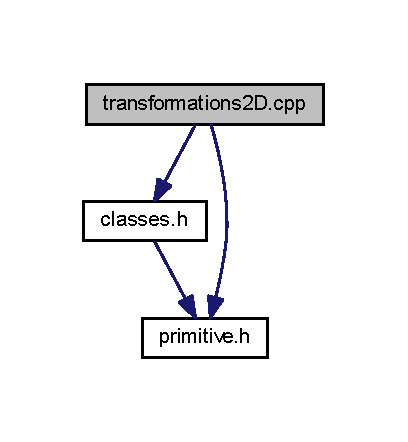
\includegraphics[width=196pt]{transformations2_d_8cpp__incl}
\end{center}
\end{figure}
\subsection*{Functions}
\begin{DoxyCompactItemize}
\item 
\mbox{\hyperlink{classobject}{object}} \mbox{\hyperlink{transformations2_d_8cpp_a6d172d5c6754ca0c9a657d3705ff765d}{Generate3D}} (\mbox{\hyperlink{classview2_d}{view2D}} a, \mbox{\hyperlink{classview2_d}{view2D}} b, \mbox{\hyperlink{classview2_d}{view2D}} c)
\item 
\mbox{\hyperlink{classview2_d}{view2D}} \mbox{\hyperlink{transformations2_d_8cpp_a6ca40087d9625015aa7c6ec2ed6af462}{translate2D}} (\mbox{\hyperlink{classview2_d}{view2D}} a, double \mbox{\hyperlink{primitive_8h_a521441fc7ec247d21ca8c376f778ff08}{x}}, double \mbox{\hyperlink{primitive_8h_a5e287957a4fe616e55aa59c129f49a92}{y}})
\item 
\mbox{\hyperlink{classview2_d}{view2D}} \mbox{\hyperlink{transformations2_d_8cpp_a05ac14eedc523383b0f5d4ebba6a5e6d}{scaling2D}} (\mbox{\hyperlink{classview2_d}{view2D}} a, double \mbox{\hyperlink{primitive_8h_a521441fc7ec247d21ca8c376f778ff08}{x}}, double \mbox{\hyperlink{primitive_8h_a5e287957a4fe616e55aa59c129f49a92}{y}})
\item 
\mbox{\hyperlink{classview2_d}{view2D}} \mbox{\hyperlink{transformations2_d_8cpp_ac598e3f9c6a0447bbd970bba10556b07}{rotation2D}} (\mbox{\hyperlink{classview2_d}{view2D}} a, int b, double c)
\end{DoxyCompactItemize}


\subsection{Function Documentation}
\mbox{\Hypertarget{transformations2_d_8cpp_a6d172d5c6754ca0c9a657d3705ff765d}\label{transformations2_d_8cpp_a6d172d5c6754ca0c9a657d3705ff765d}} 
\index{transformations2\+D.\+cpp@{transformations2\+D.\+cpp}!Generate3D@{Generate3D}}
\index{Generate3D@{Generate3D}!transformations2\+D.\+cpp@{transformations2\+D.\+cpp}}
\subsubsection{\texorpdfstring{Generate3\+D()}{Generate3D()}}
{\footnotesize\ttfamily \mbox{\hyperlink{classobject}{object}} Generate3D (\begin{DoxyParamCaption}\item[{\mbox{\hyperlink{classview2_d}{view2D}}}]{a,  }\item[{\mbox{\hyperlink{classview2_d}{view2D}}}]{b,  }\item[{\mbox{\hyperlink{classview2_d}{view2D}}}]{c }\end{DoxyParamCaption})}

\mbox{\Hypertarget{transformations2_d_8cpp_ac598e3f9c6a0447bbd970bba10556b07}\label{transformations2_d_8cpp_ac598e3f9c6a0447bbd970bba10556b07}} 
\index{transformations2\+D.\+cpp@{transformations2\+D.\+cpp}!rotation2D@{rotation2D}}
\index{rotation2D@{rotation2D}!transformations2\+D.\+cpp@{transformations2\+D.\+cpp}}
\subsubsection{\texorpdfstring{rotation2\+D()}{rotation2D()}}
{\footnotesize\ttfamily \mbox{\hyperlink{classview2_d}{view2D}} rotation2D (\begin{DoxyParamCaption}\item[{\mbox{\hyperlink{classview2_d}{view2D}}}]{a,  }\item[{int}]{b,  }\item[{double}]{c }\end{DoxyParamCaption})}

\mbox{\Hypertarget{transformations2_d_8cpp_a05ac14eedc523383b0f5d4ebba6a5e6d}\label{transformations2_d_8cpp_a05ac14eedc523383b0f5d4ebba6a5e6d}} 
\index{transformations2\+D.\+cpp@{transformations2\+D.\+cpp}!scaling2D@{scaling2D}}
\index{scaling2D@{scaling2D}!transformations2\+D.\+cpp@{transformations2\+D.\+cpp}}
\subsubsection{\texorpdfstring{scaling2\+D()}{scaling2D()}}
{\footnotesize\ttfamily \mbox{\hyperlink{classview2_d}{view2D}} scaling2D (\begin{DoxyParamCaption}\item[{\mbox{\hyperlink{classview2_d}{view2D}}}]{a,  }\item[{double}]{x,  }\item[{double}]{y }\end{DoxyParamCaption})}

\mbox{\Hypertarget{transformations2_d_8cpp_a6ca40087d9625015aa7c6ec2ed6af462}\label{transformations2_d_8cpp_a6ca40087d9625015aa7c6ec2ed6af462}} 
\index{transformations2\+D.\+cpp@{transformations2\+D.\+cpp}!translate2D@{translate2D}}
\index{translate2D@{translate2D}!transformations2\+D.\+cpp@{transformations2\+D.\+cpp}}
\subsubsection{\texorpdfstring{translate2\+D()}{translate2D()}}
{\footnotesize\ttfamily \mbox{\hyperlink{classview2_d}{view2D}} translate2D (\begin{DoxyParamCaption}\item[{\mbox{\hyperlink{classview2_d}{view2D}}}]{a,  }\item[{double}]{x,  }\item[{double}]{y }\end{DoxyParamCaption})}


\hypertarget{transformations3_d_8cpp}{}\section{transformations3\+D.\+cpp File Reference}
\label{transformations3_d_8cpp}\index{transformations3\+D.\+cpp@{transformations3\+D.\+cpp}}
{\ttfamily \#include \char`\"{}classes.\+h\char`\"{}}\newline
{\ttfamily \#include \char`\"{}primitive.\+h\char`\"{}}\newline
Include dependency graph for transformations3\+D.\+cpp\+:
\nopagebreak
\begin{figure}[H]
\begin{center}
\leavevmode
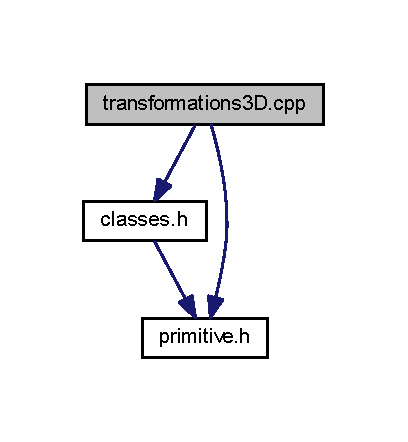
\includegraphics[width=196pt]{transformations3_d_8cpp__incl}
\end{center}
\end{figure}
\subsection*{Functions}
\begin{DoxyCompactItemize}
\item 
\mbox{\hyperlink{classobject}{object}} \mbox{\hyperlink{transformations3_d_8cpp_a826c89a0dfa35158ea10672dddc46ebb}{translate3D}} (\mbox{\hyperlink{classobject}{object}} a, double \mbox{\hyperlink{primitive_8h_a521441fc7ec247d21ca8c376f778ff08}{x}}, double \mbox{\hyperlink{primitive_8h_a5e287957a4fe616e55aa59c129f49a92}{y}}, double \mbox{\hyperlink{primitive_8h_aa4b230975c7672e64e45f871e10cddc1}{z}})
\item 
\mbox{\hyperlink{classobject}{object}} \mbox{\hyperlink{transformations3_d_8cpp_a5637b9751b633dbc13b5eae664fa6871}{scaling3D}} (\mbox{\hyperlink{classobject}{object}} a, double \mbox{\hyperlink{primitive_8h_a521441fc7ec247d21ca8c376f778ff08}{x}}, double \mbox{\hyperlink{primitive_8h_a5e287957a4fe616e55aa59c129f49a92}{y}}, double \mbox{\hyperlink{primitive_8h_aa4b230975c7672e64e45f871e10cddc1}{z}})
\item 
\mbox{\hyperlink{classobject}{object}} \mbox{\hyperlink{transformations3_d_8cpp_aec010ce043d90235911569b3404bc843}{reflection3D}} (\mbox{\hyperlink{classobject}{object}} a, int b)
\item 
\mbox{\hyperlink{classobject}{object}} \mbox{\hyperlink{transformations3_d_8cpp_a783c292415ebe3034ab64864e9e2b13f}{rotation3D}} (\mbox{\hyperlink{classobject}{object}} a, vertex3D v, \mbox{\hyperlink{classedge3_d}{edge3D}} e, int i, double o)
\end{DoxyCompactItemize}


\subsection{Function Documentation}
\mbox{\Hypertarget{transformations3_d_8cpp_aec010ce043d90235911569b3404bc843}\label{transformations3_d_8cpp_aec010ce043d90235911569b3404bc843}} 
\index{transformations3\+D.\+cpp@{transformations3\+D.\+cpp}!reflection3D@{reflection3D}}
\index{reflection3D@{reflection3D}!transformations3\+D.\+cpp@{transformations3\+D.\+cpp}}
\subsubsection{\texorpdfstring{reflection3\+D()}{reflection3D()}}
{\footnotesize\ttfamily \mbox{\hyperlink{classobject}{object}} reflection3D (\begin{DoxyParamCaption}\item[{\mbox{\hyperlink{classobject}{object}}}]{a,  }\item[{int}]{b }\end{DoxyParamCaption})}

\mbox{\Hypertarget{transformations3_d_8cpp_a783c292415ebe3034ab64864e9e2b13f}\label{transformations3_d_8cpp_a783c292415ebe3034ab64864e9e2b13f}} 
\index{transformations3\+D.\+cpp@{transformations3\+D.\+cpp}!rotation3D@{rotation3D}}
\index{rotation3D@{rotation3D}!transformations3\+D.\+cpp@{transformations3\+D.\+cpp}}
\subsubsection{\texorpdfstring{rotation3\+D()}{rotation3D()}}
{\footnotesize\ttfamily \mbox{\hyperlink{classobject}{object}} rotation3D (\begin{DoxyParamCaption}\item[{\mbox{\hyperlink{classobject}{object}}}]{a,  }\item[{vertex3D}]{v,  }\item[{\mbox{\hyperlink{classedge3_d}{edge3D}}}]{e,  }\item[{int}]{i,  }\item[{double}]{o }\end{DoxyParamCaption})}

\mbox{\Hypertarget{transformations3_d_8cpp_a5637b9751b633dbc13b5eae664fa6871}\label{transformations3_d_8cpp_a5637b9751b633dbc13b5eae664fa6871}} 
\index{transformations3\+D.\+cpp@{transformations3\+D.\+cpp}!scaling3D@{scaling3D}}
\index{scaling3D@{scaling3D}!transformations3\+D.\+cpp@{transformations3\+D.\+cpp}}
\subsubsection{\texorpdfstring{scaling3\+D()}{scaling3D()}}
{\footnotesize\ttfamily \mbox{\hyperlink{classobject}{object}} scaling3D (\begin{DoxyParamCaption}\item[{\mbox{\hyperlink{classobject}{object}}}]{a,  }\item[{double}]{x,  }\item[{double}]{y,  }\item[{double}]{z }\end{DoxyParamCaption})}

\mbox{\Hypertarget{transformations3_d_8cpp_a826c89a0dfa35158ea10672dddc46ebb}\label{transformations3_d_8cpp_a826c89a0dfa35158ea10672dddc46ebb}} 
\index{transformations3\+D.\+cpp@{transformations3\+D.\+cpp}!translate3D@{translate3D}}
\index{translate3D@{translate3D}!transformations3\+D.\+cpp@{transformations3\+D.\+cpp}}
\subsubsection{\texorpdfstring{translate3\+D()}{translate3D()}}
{\footnotesize\ttfamily \mbox{\hyperlink{classobject}{object}} translate3D (\begin{DoxyParamCaption}\item[{\mbox{\hyperlink{classobject}{object}}}]{a,  }\item[{double}]{x,  }\item[{double}]{y,  }\item[{double}]{z }\end{DoxyParamCaption})}


%--- End generated contents ---

% Index
\backmatter
\newpage
\phantomsection
\clearemptydoublepage
\addcontentsline{toc}{chapter}{Index}
\printindex

\end{document}
